Three main sources of SM background can be distinguished in this analysis. 
A first category consists of events with two same-sign prompt leptons or at least three prompt leptons, 
mainly from $\ttbar V$ and diboson processes. 
Other types of background events include those containing electrons with mis-measured charge, mainly from the production of top quark pairs, 
and those containing at least one non-prompt or fake lepton, 
which mainly originate from hadron decays in events containing top quarks or of $W$ bosons in association with jets. 

\subsection{Background estimation methods} 

The estimation of the SM background processes with two same-sign prompt leptons or at least three prompt leptons 
is performed using the MC samples described in Section~\ref{sec:dataMC}. 
Since diboson and $\ttbar V$ events are the main backgrounds in the signal regions, 
dedicated validation regions with an enhanced contribution from these processes 
are defined to verify the background predictions (see Section~\ref{sec:valid}).

Background events due to charge mis-identification, dominated by electrons having emitted 
a hard brems\-strah\-lung photon which subsequently converted to an electron--positron pair, 
are referred to as “charge-flip”. 
The probability of mis-identifying the charge of a muon is checked in both data and MC simulation, 
and found to be negligible in the kinematic range relevant to this analysis.
The contribution of charge-flip events is estimated using data. 
The electron charge-flip probability is extracted in a $Z/\gamma^{*}\to ee$ data sample using a likelihood fit 
which takes as input the numbers of same-sign and opposite-sign electron pairs observed in the sample. 
The charge-flip probability is a free parameter of the fit and is extracted as a function of the electron $\pt$ and $\eta$. 
The event yield of this background in the signal or validation regions is obtained by applying the measured charge-flip probability 
to data regions with the same kinematic requirements as the signal or validation regions but with opposite-sign lepton pairs. 


The contribution from fake or non-prompt (FNP) leptons (such as hadrons mis-identified as leptons, 
leptons originating from heavy-flavour decays, and electrons from photon conversions) 
is also estimated from data with a matrix method similar to that described in Ref.~\cite{paperSS3L}. 
In this method, two types of lepton identification criteria are defined: ``tight'', 
corresponding to the signal lepton criteria described in Section~\ref{sec:selection}, 
and ``loose'', corresponding to candidate leptons. 
The matrix method relates the number of events containing prompt or FNP leptons 
to the number of observed events with tight or loose-not-tight leptons 
using the probability for loose prompt or FNP leptons to satisfy the tight criteria. 
The probability for loose prompt leptons to satisfy the tight selection criteria 
is obtained using a $Z/\gamma^*\to\ell\ell$ data sample 
and is modelled as a function of the lepton $\pt$ and $\eta$. 
The probability for loose FNP leptons to satisfy the tight selection criteria is determined from data 
in a SS control region enriched in non-prompt leptons originating from heavy-flavour decays. 
This region contains events with at least one $b$-jet, 
one tight muon with $\pt > \SI{40}{GeV}$ (likely prompt) and an additional loose electron or muon (likely FNP).
The contribution from prompt leptons and charge mis-measured electrons to this region is subtracted from the observed event yields.

The data-driven background estimates are cross-checked with an MC-based technique. 
In this method, the contributions from processes with FNP leptons and electron charge mis-identification 
are obtained from MC simulation and normalised to data in dedicated control regions at low jet multiplicity, low $\met$, and 
either with or without $b$-jets. 
The normalisation is performed using five multipliers: one to correct 
the electron charge mis-identification rate, and four to correct the contributions from FNP 
electrons or muons originating from $b$-jets or light-flavour jets, respectively.
In addition to the MC samples listed in Section~\ref{sec:dataMC}, this method employs samples of top quark pair production generated with the \POWHEG-Box v2 generator interfaced to \PYTHIA 6.428~\cite{Sjostrand:2006za}, 
as well as samples of simulated $W$+jets and $Z$+jets events generated with \POWHEG-Box v2 interfaced to \PYTHIA 8.186.

\subsection{Systematic uncertainties on the background estimation}

Table~\ref{tab:SR_syst} summarises the contributions of the different sources of systematic uncertainty 
in the total SM background predictions in the signal regions.

The systematic uncertainties related to the same-sign prompt leptons background estimation 
arise from the accuracy of the theoretical and experimental modelling in the MC simulation.
The primary sources of systematic uncertainties are related to
the jet energy scale calibration, 
the jet energy resolution, 
$b$-tagging efficiency, 
and MC modelling and theoretical cross-section uncertainties. 
The cross-sections used to normalise the MC samples are varied according to the uncertainty in the 
cross-section calculation, that is, 6\% for diboson, 13\% for $\ttbar W$ and 12\% $\ttbar Z$ production~\cite{Alwall:2014hca}.
Additional uncertainties are assigned to these backgrounds 
to account for the modelling of the kinematic distributions in the MC simulation. 
For $\ttbar W$ and $\ttbar Z$, the predictions from the \MADGRAPH and \SHERPA generators are compared, 
leading to a $\sim$30\% uncertainty for these processes after the SR selections. 
For dibosons, uncertainties are estimated by varying the renormalisation, factorisation and resummation scales used to generate these samples, 
leading to a $\sim$30\% uncertainty for these processes after the SR selections. 
For triboson, $\ttbar h$, $\ttbar \ttbar$ and $tZ$ production processes, which constitute a small background in all signal regions, a 50\% uncertainty on the event yields is assumed.

Uncertainties in the FNP lepton background estimate are assigned due to the limited number of data events with loose and tight leptons.
In addition, systematic uncertainties of 50--60\% are assigned to the probabilities for loose FNP leptons to satisfy the tight signal criteria to account for potentially different FNP compositions (heavy flavour, light flavour or conversions) between the regions used to measure these probabilities and the SRs, as well as the contamination from prompt leptons in the former regions.
This leads to overall FNP background uncertainties in the total background estimates of 18--21\% depending on the signal region.

For the charge-flip background prediction, the main uncertainties originate from the statistical 
uncertainty of the charge-flip probability measurements and the background contamination of the 
sample used to extract the charge-flip probability. 

\begin{table}[h!]
\begin{center}
\caption{The main sources of systematic uncertainty on the SM background estimates for the four signal regions are shown 
and their values given as relative uncertainties in the expected signal region background event yields. 
The individual components can be correlated and therefore do not necessarily add up in quadrature to the total systematic uncertainty.
For reference, the total number of expected background events is also shown.
}
\label{tab:SR_syst}
{\small
\begin{tabular}{lrrrr}
\noalign{\smallskip}\hline\hline\noalign{\smallskip}
         & SR0b3j         & SR0b5j     & SR1b & SR3b     \\[-0.05cm]
\noalign{\smallskip}\hline\hline\noalign{\smallskip}
Diboson theoretical uncertainties    & 23\%  &  16\%   &  1\%  &$<$1\%   \\
$\ttbar V$ theoretical uncertainties & 3\%   &  4\%    & 13\%  &  9\%   \\
Other theoretical uncertainties      & 5\%   &  3\%    &  9\%  & 15\%   \\
\noalign{\smallskip}\hline\noalign{\smallskip}
MC statistical uncertainties         & 11\%  &  14\%   &  3\%  &  6\%   \\
\noalign{\smallskip}\hline\noalign{\smallskip}
Jet energy scale        & 12\%   &  11\%  & 6\%    & 5\%   \\
Jet energy resolution   & 3\%    &  9\%   & 2\%    & 3\%   \\
$b$-tagging             & 4\%    &  6\%   & 3\%    & 10\%   \\
PDF                     & 6\%    &  6\%   & 6\%    & 8\%   \\
Fake/non-prompt leptons & 18\%    &  20\%   & 18\%   & 21\%   \\
Charge flip             & --     & 1\% & 3\%    & 8\%   \\
\noalign{\smallskip}\hline\noalign{\smallskip}
Total background uncertainties & 30\%   & 34\%   & 22\%   & 31\%   \\
\noalign{\smallskip}\hline\hline\noalign{\smallskip}
Total background events & $1.5$ & $0.88$ & $4.5$ & $0.80$\\
\noalign{\smallskip}\hline\hline\noalign{\smallskip}
\end{tabular}
}
\end{center}
\end{table}

\subsection{Validation of background estimates}
\label{sec:valid}

To check the validity and robustness of the background estimates, 
the distributions of several discriminating variables in data are compared 
with the predicted background after various requirements on the number of jets and $b$-jets. 
Events are categorised based on the flavours of the selected leptons, and the different flavour channels are compared separately. 
Examples of such distributions are shown in Fig.~\ref{fig:VRa}--\ref{fig:VRc}
and illustrate that the predictions and data agree fairly well. 
The background estimates in a kinematic region close to the signal regions can also be observed in Fig.~\ref{fig:Results_SR_metD}, 
which shows the \met distributions in the signal regions before applying the \met requirements. 

\begin{table}[t!]
\caption{Summary of the event selection in the validation regions. 
Requirements are placed on the number of signal leptons ($N_{\rm{lept}}^{\rm{signal}}$) and candidate leptons ($N_{\rm{lept}}^{\rm{cand}}$), 
the number of jets with $\pt>\SI{25}{GeV}$ ($N_{\rm{jets}}^{25}$) or the number of $b$-jets with $\pt>\SI{20}{GeV}$ ($N_{b\rm{-jets}}^{20}$). 
The three leading-\pt leptons are referred to as $\ell_{1,2,3}$ with decreasing \pt and the two leading jets as $j_{1,2}$.
Additional requirements are set on the invariant mass of the two leading electrons $m_{ee}$, 
the presence of SS leptons or a pair of same-flavour opposite-sign leptons (SFOS) and its invariant mass $m_\text{SFOS}$. 
}
\hspace{0.5cm}
\def\arraystretch{1.1}
\label{tab:VRdef}
\centering
\resizebox{\textwidth}{!}
{\small
\begin{tabular}{c|c|c|c|c|c|l}
\hline 
\hline    
          &  $N_{\rm{lept}}^{\rm{signal}}$ ($N_{\rm{lept}}^{\rm{cand}}$)   & $N_{b\rm{-jets}}^{20}$  &  $N_{\rm{jets}}^{25}$  & \met\ [GeV] & \meff\ [GeV]  & Other \\
\hline\hline
VR-WW   & =2 (=2) &  =0  &  $\geq$2 & 35--200  & 300--900 & $m(j_1 j_2)>500$~GeV\\
          & =1 SS pair    &      &             &         &         & $\pt(j_2)>40$~GeV\\
          &      &      &             &         &         & $\pt(\ell_2)>30$~GeV\\
          &      &      &             &         &         & veto $80<m_{ee}<100$~GeV \\\hline
VR-WZ     & =3 (=3) &  =0  &  1--3     & 30--200  & $<$900 & $\pt(\ell_3)>30$~GeV \\ \hline
VR-ttV    &$\geq$2 (-) &$\geq$2&  $\geq$5 ($e^\pm e^\pm$,$e^\pm \mu^\pm$) & 20--200  & 200--900 & $\pt(\ell_2)>25$~GeV\\
          & $\geq$1 SS pair  &         &  $\geq$3 ($\mu^\pm \mu^\pm$)             &          &         & veto $\{\met>125$ and $\meff>\SI{650}{GeV}\}$\\ \hline
VR-ttZ    &$\geq$3 (-) & $\geq$1 & $\geq$4 ($=$1 $b$-jet)         & 20--150  & 100--900 & $\pt(\ell_2)>25$~GeV\\
          &$\geq$1 SFOS pair &         & $\geq$3 ($\geq$2 $b$-jets) &           &     & $\pt(\ell_3)>20$~GeV (if $e$)\\
          &        &         &                           &          &         & $80<m_\text{SFOS}<100$~GeV \\
\hline\hline
All VRs & \multicolumn{6}{c}{Veto events belonging to any SR, or if $\ell_1$ or $\ell_2$ is an electron with $|\eta|>1.37$ (except in VR-WZ)}\\
\hline\hline
\end{tabular}
}
\end{table}

Dedicated validation regions (VRs) are defined to test the estimate of the rare SM processes contributing to the signal regions, 
whose cross-sections have not yet been measured at $\sqrt s=13$ TeV. 
The corresponding selections are summarised in Table~\ref{tab:VRdef}. 
In these regions, upper bounds are placed on \met and \meff{} to reduce signal contamination, 
and the small residual overlap with the signal regions is resolved by vetoing events that contribute to the signal regions.  
To further reduce contributions from electron charge mis-identification, 
events are also vetoed if one of the two leading leptons is an electron with $|\eta|>1.37$, 
since contributions from charge-flip electrons are smaller in the central region due to the lower amount of crossed material. 
The purity of the targeted processes in these regions ranges from about 40\% to $80\%$. 
The VR-ttV and VR-ttZ regions overlap with each other, with 30\% of the $\ttbar V$ events in VR-ttV 
also present in VR-ttZ, 
and the contributions from the $\ttbar Z$ and $\ttbar W$ processes is similar in VR-ttV.


The observed yields in these validation regions, compared with the background predictions and uncertainties, 
can be seen in Table~\ref{tab:VR_yields}, and the effective mass distributions are shown in Fig.~\ref{fig:VRd}--\ref{fig:VRf}.
There is fair agreement between data and the estimated background for the validation regions, 
with the largest deviations being observed in VR-ttV with a 1.5$\sigma$ deviation. 


\begin{table}
\caption{The numbers of observed data and expected background events for the validation regions. 
The ``Rare'' category contains the contributions from associated production of $\ttbar$ with $h/WW/t/\ttbar$, 
as well as $tZ$, $Wh$, $Zh$, and triboson production. 
Background categories shown as ``$-$'' denote that they cannot contribute to a given region (charge flips or $W^\pm W^\pm jj$ in 3-lepton regions). 
The individual uncertainties can be correlated and therefore do not necessarily add up in quadrature to the total systematic uncertainty. }
\label{tab:VR_yields}
\begin{center}
\setlength{\tabcolsep}{0.0pc}
{\small
\begin{tabular*}{\textwidth}{@{\extracolsep{\fill}}lcccc}
\noalign{\smallskip}\hline\hline\noalign{\smallskip}
          & VR-WW       & VR-WZ     & VR-ttV  & VR-ttZ     \\[-0.05cm]
\noalign{\smallskip}\hline\hline\noalign{\smallskip}
Observed events          & $4$       &  $82$   & $19$  & $14$ \\
\noalign{\smallskip}\hline\noalign{\smallskip}
Total background events & $3.4 \pm 0.8$ & $98 \pm 15$ & $12.1 \pm 2.7$\hspace*{1.75mm} & $9.7 \pm 2.5$\\
\noalign{\smallskip}\hline\noalign{\smallskip}
Fake/non-prompt leptons & $0.6 \pm 0.5$ & $8 \pm 6$ & $2.1 \pm 1.4$ & $0.6\pm 1.0$\\ 
Charge-flip & $0.26 \pm 0.05$ & $-$ & $1.14 \pm 0.15$ & $-$\\
$t\bar{t}W$ & $0.05 \pm 0.03$ & $0.25 \pm 0.09$ & $2.4 \pm 0.8$ & $0.10 \pm 0.03$\\
$t\bar{t}Z$ & $0.02 \pm 0.01$ & $0.72 \pm 0.26$ & $3.9 \pm 1.3$ & $6.3 \pm 2.1$\\
$WZ$ & $1.0 \pm 0.4$ & $78 \pm 13$ & $0.19 \pm 0.10$ & $1.2 \pm 0.4$\\
$W^\pm W^\pm jj$ & $1.3 \pm 0.5$ & $-$ & $0.02 \pm 0.03$ & $-$\\
$ZZ$ & $0.02 \pm 0.01$ & $8.2 \pm 2.8$ & $0.12 \pm 0.15$ & $0.30 \pm 0.19$\\
Rare & $0.10 \pm 0.05$ & $2.8 \pm 1.4$ & $2.3 \pm 1.2$ & $1.1 \pm 0.6$\\
\noalign{\smallskip}\hline\hline\noalign{\smallskip}
\end{tabular*}
}
\end{center}
\end{table}
		
		
\begin{figure}[p!]
\centering
\begin{subfigure}[t]{0.46\textwidth}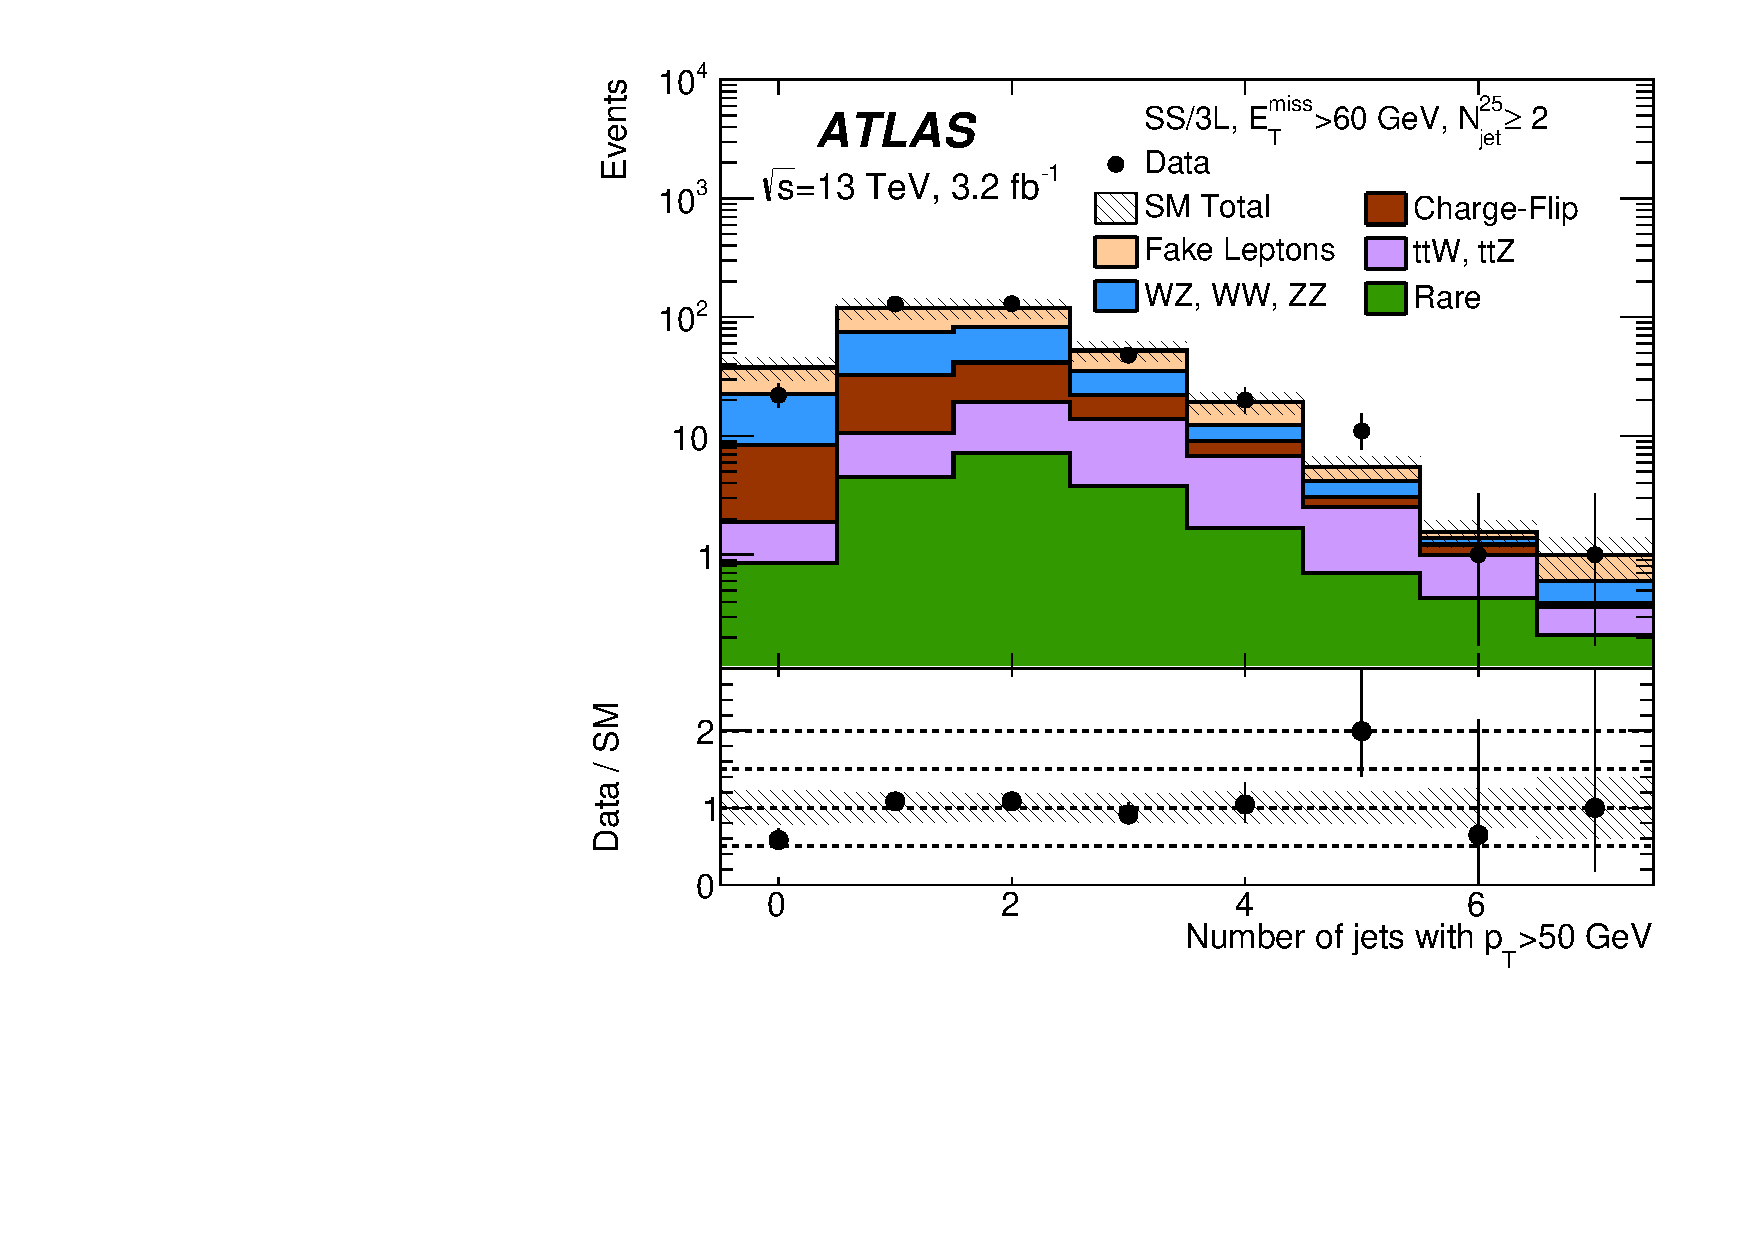
\includegraphics[width=\textwidth]{FIGURES/CONF_LEP_LEP_NJETS50.pdf}
\caption{}\label{fig:VRa}\end{subfigure}
\begin{subfigure}[t]{0.46\textwidth}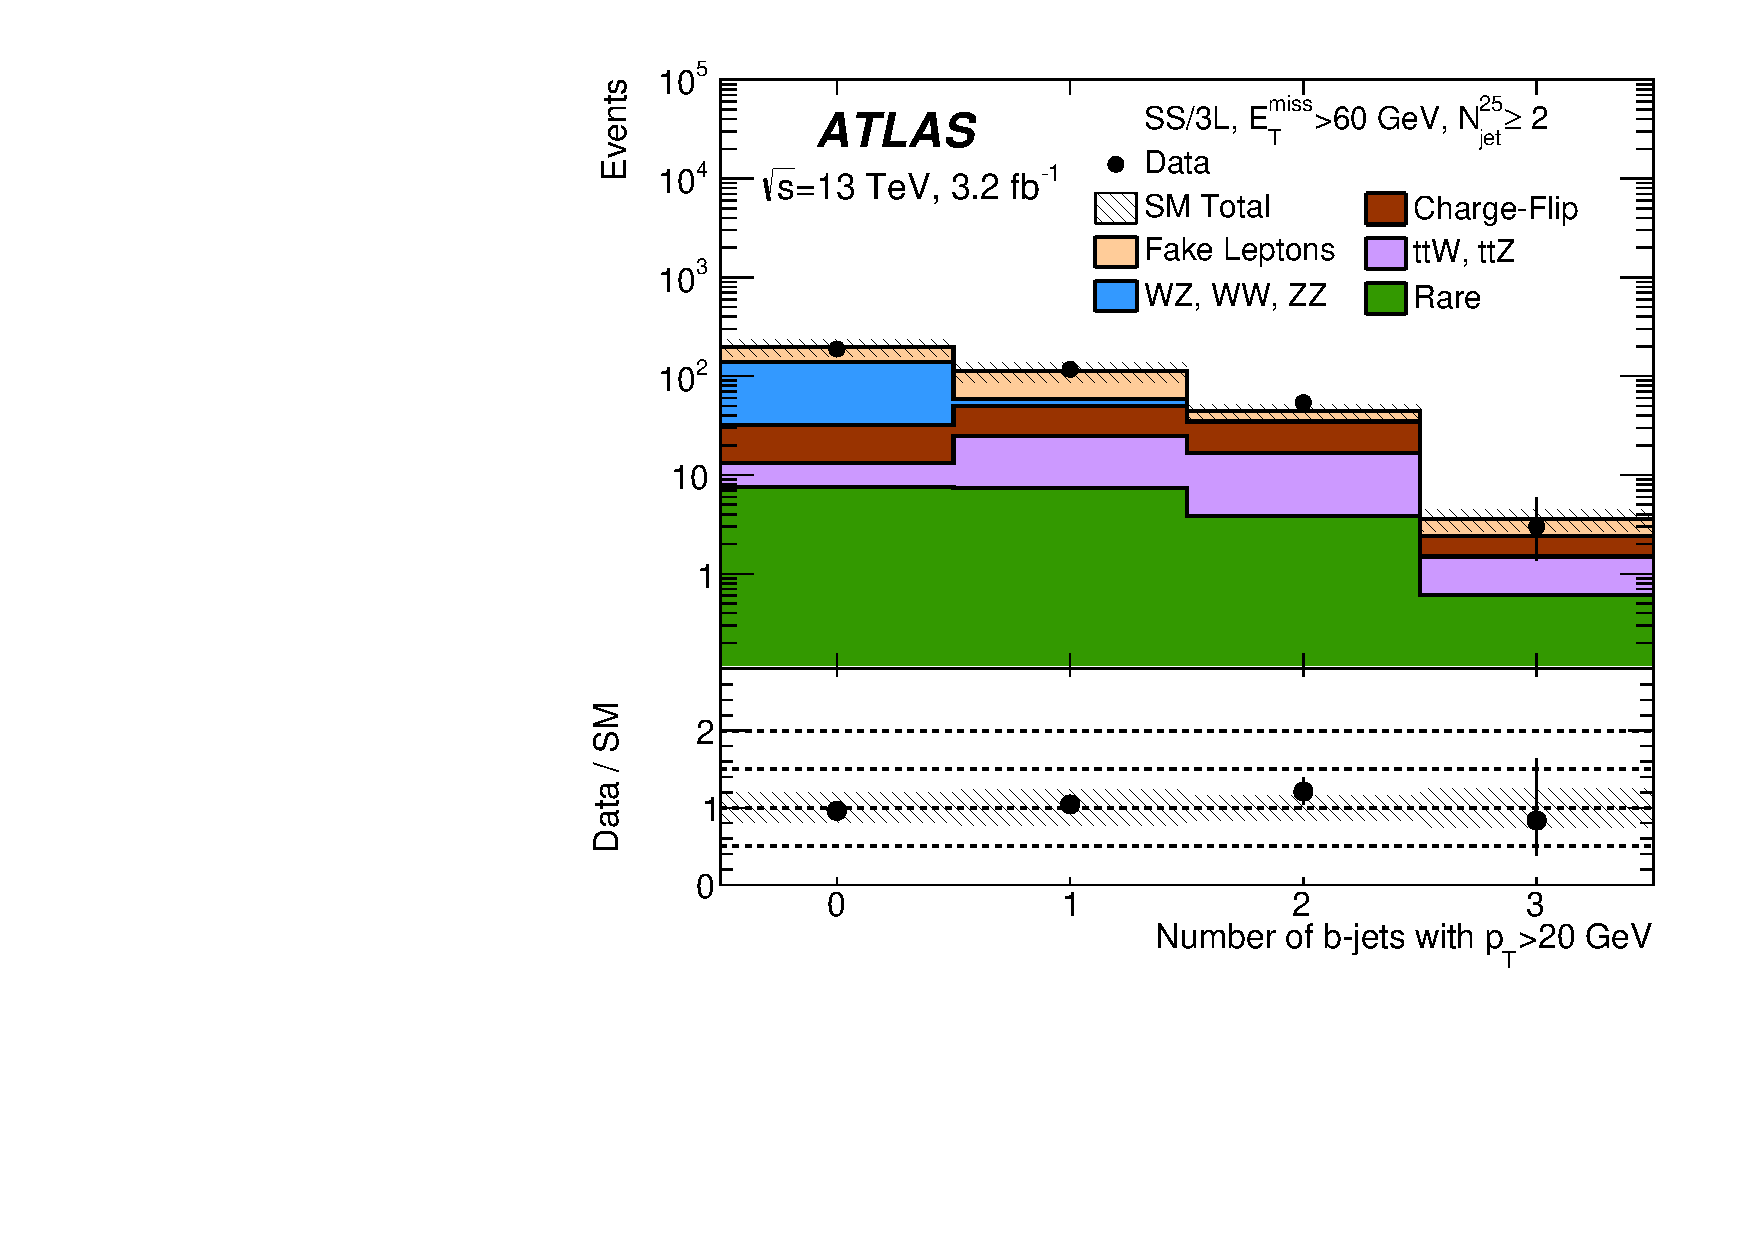
\includegraphics[width=\textwidth]{FIGURES/CONF_LEP_NBJETS20.pdf}
\caption{}\label{fig:VRb}\end{subfigure}
\begin{subfigure}[t]{0.46\textwidth}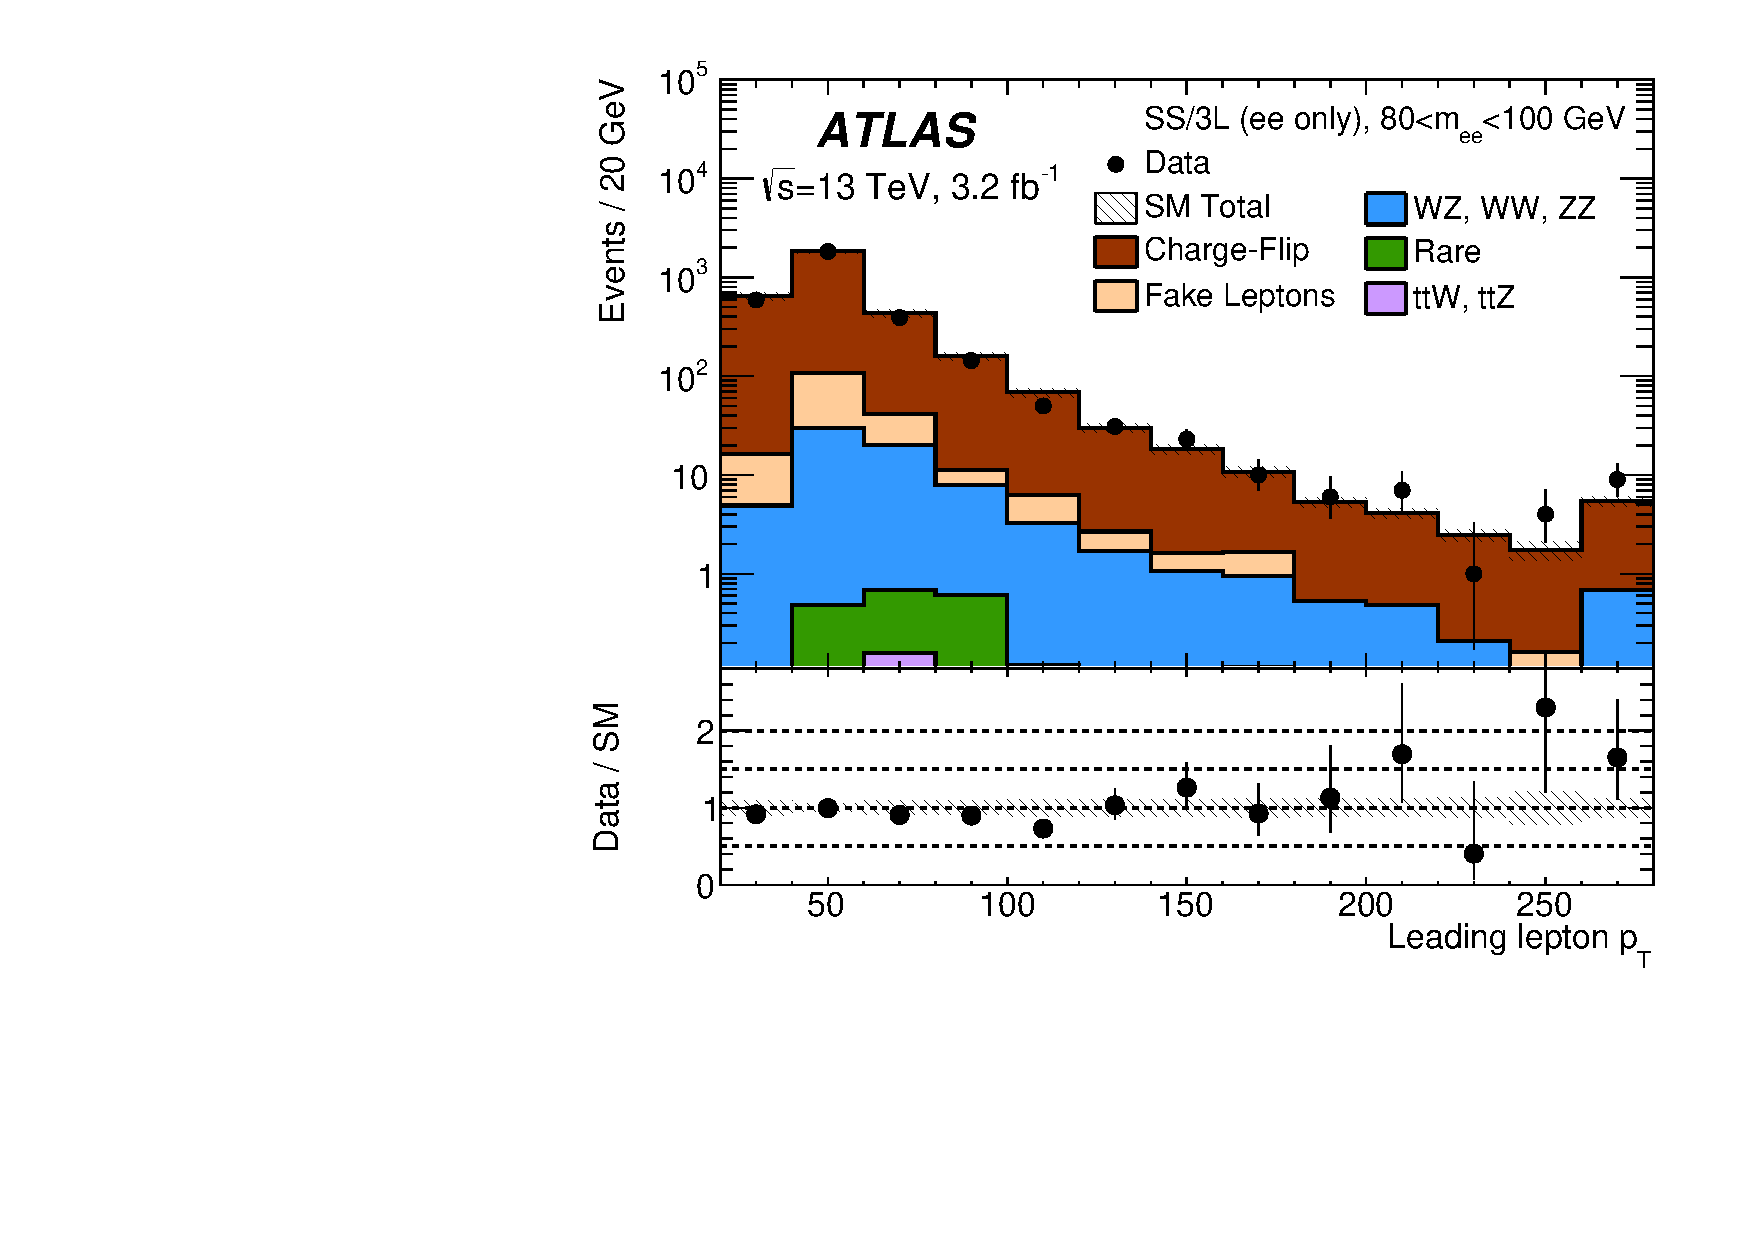
\includegraphics[width=\textwidth]{FIGURES/CONF_EE_ZcutBveto_PTLEAD.pdf}
\caption{}\label{fig:VRc}\end{subfigure}
\begin{subfigure}[t]{0.46\textwidth}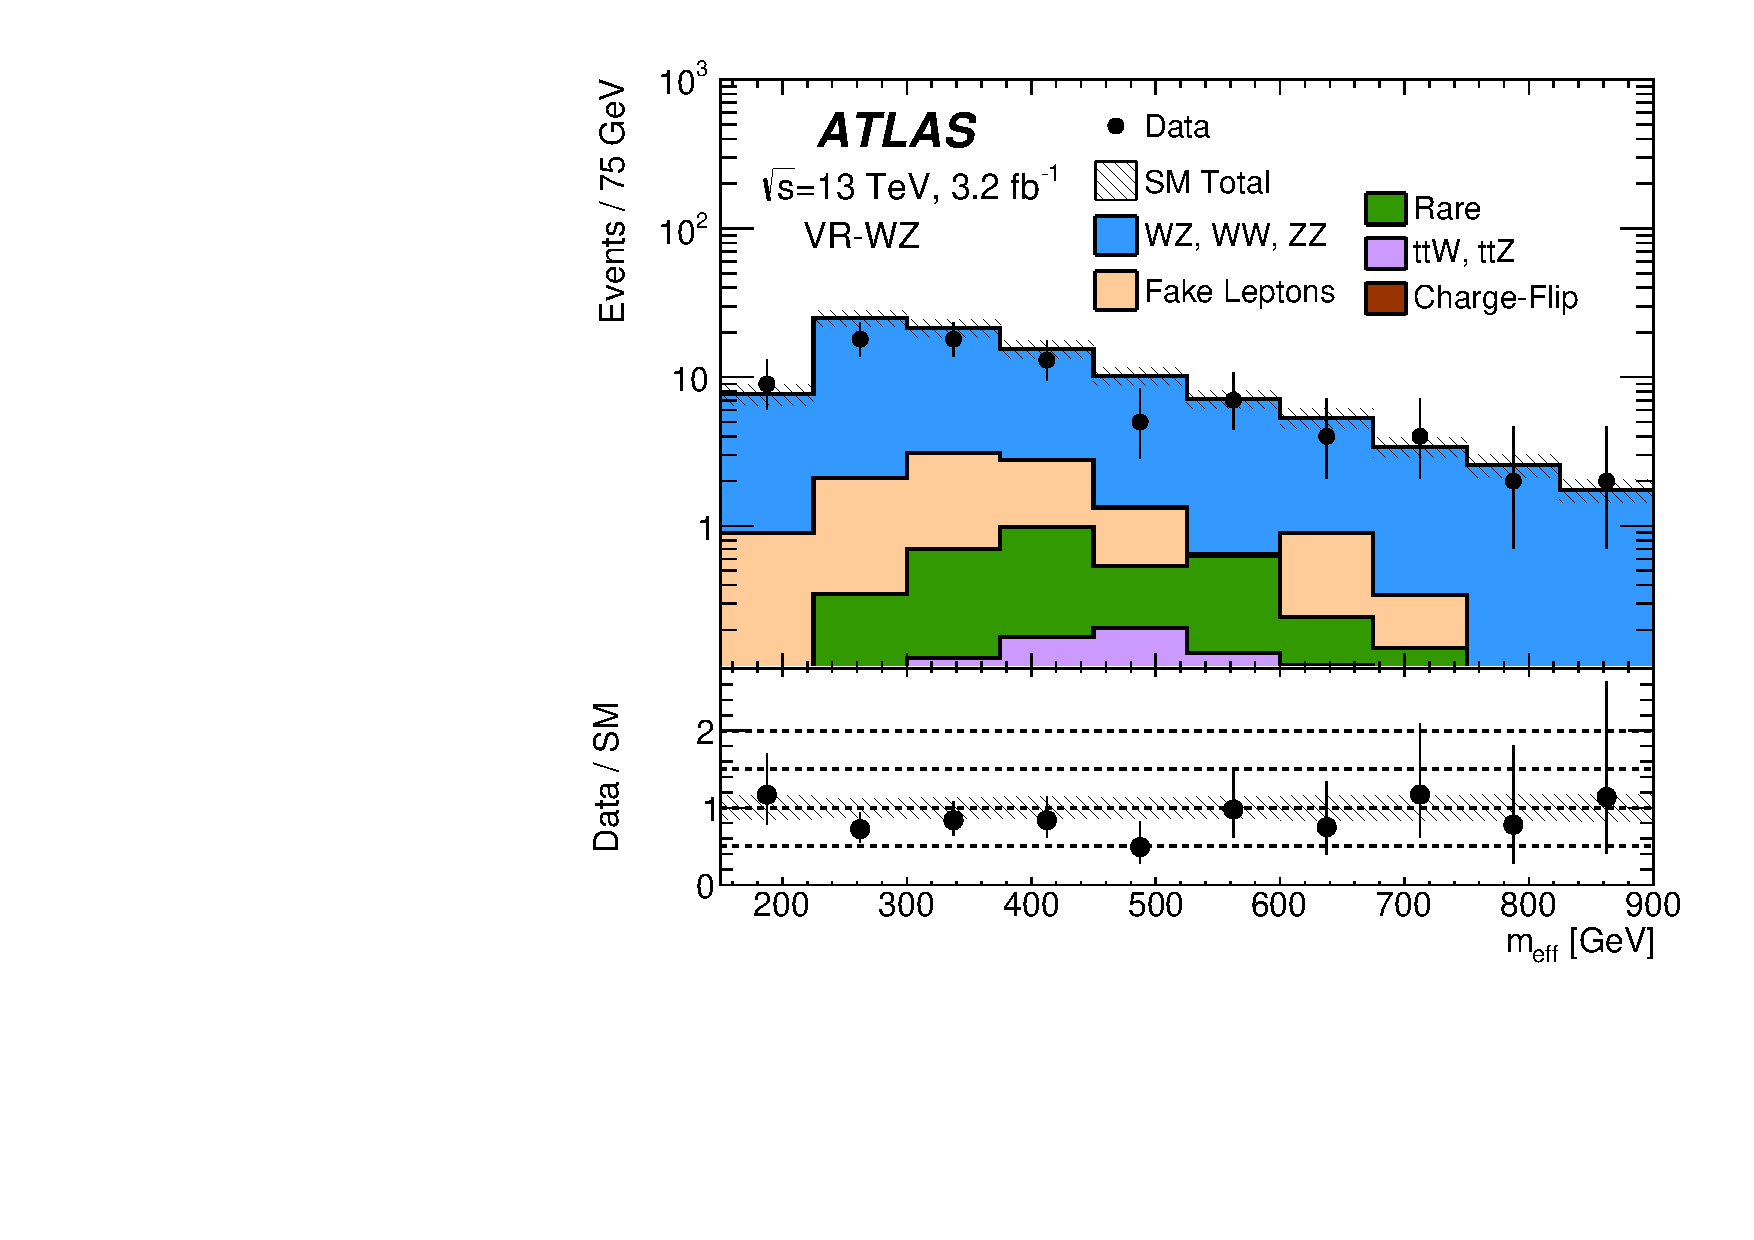
\includegraphics[width=\textwidth]{FIGURES/CONF_WZVR.pdf}
\caption{}\label{fig:VRd}\end{subfigure}
\begin{subfigure}[t]{0.46\textwidth}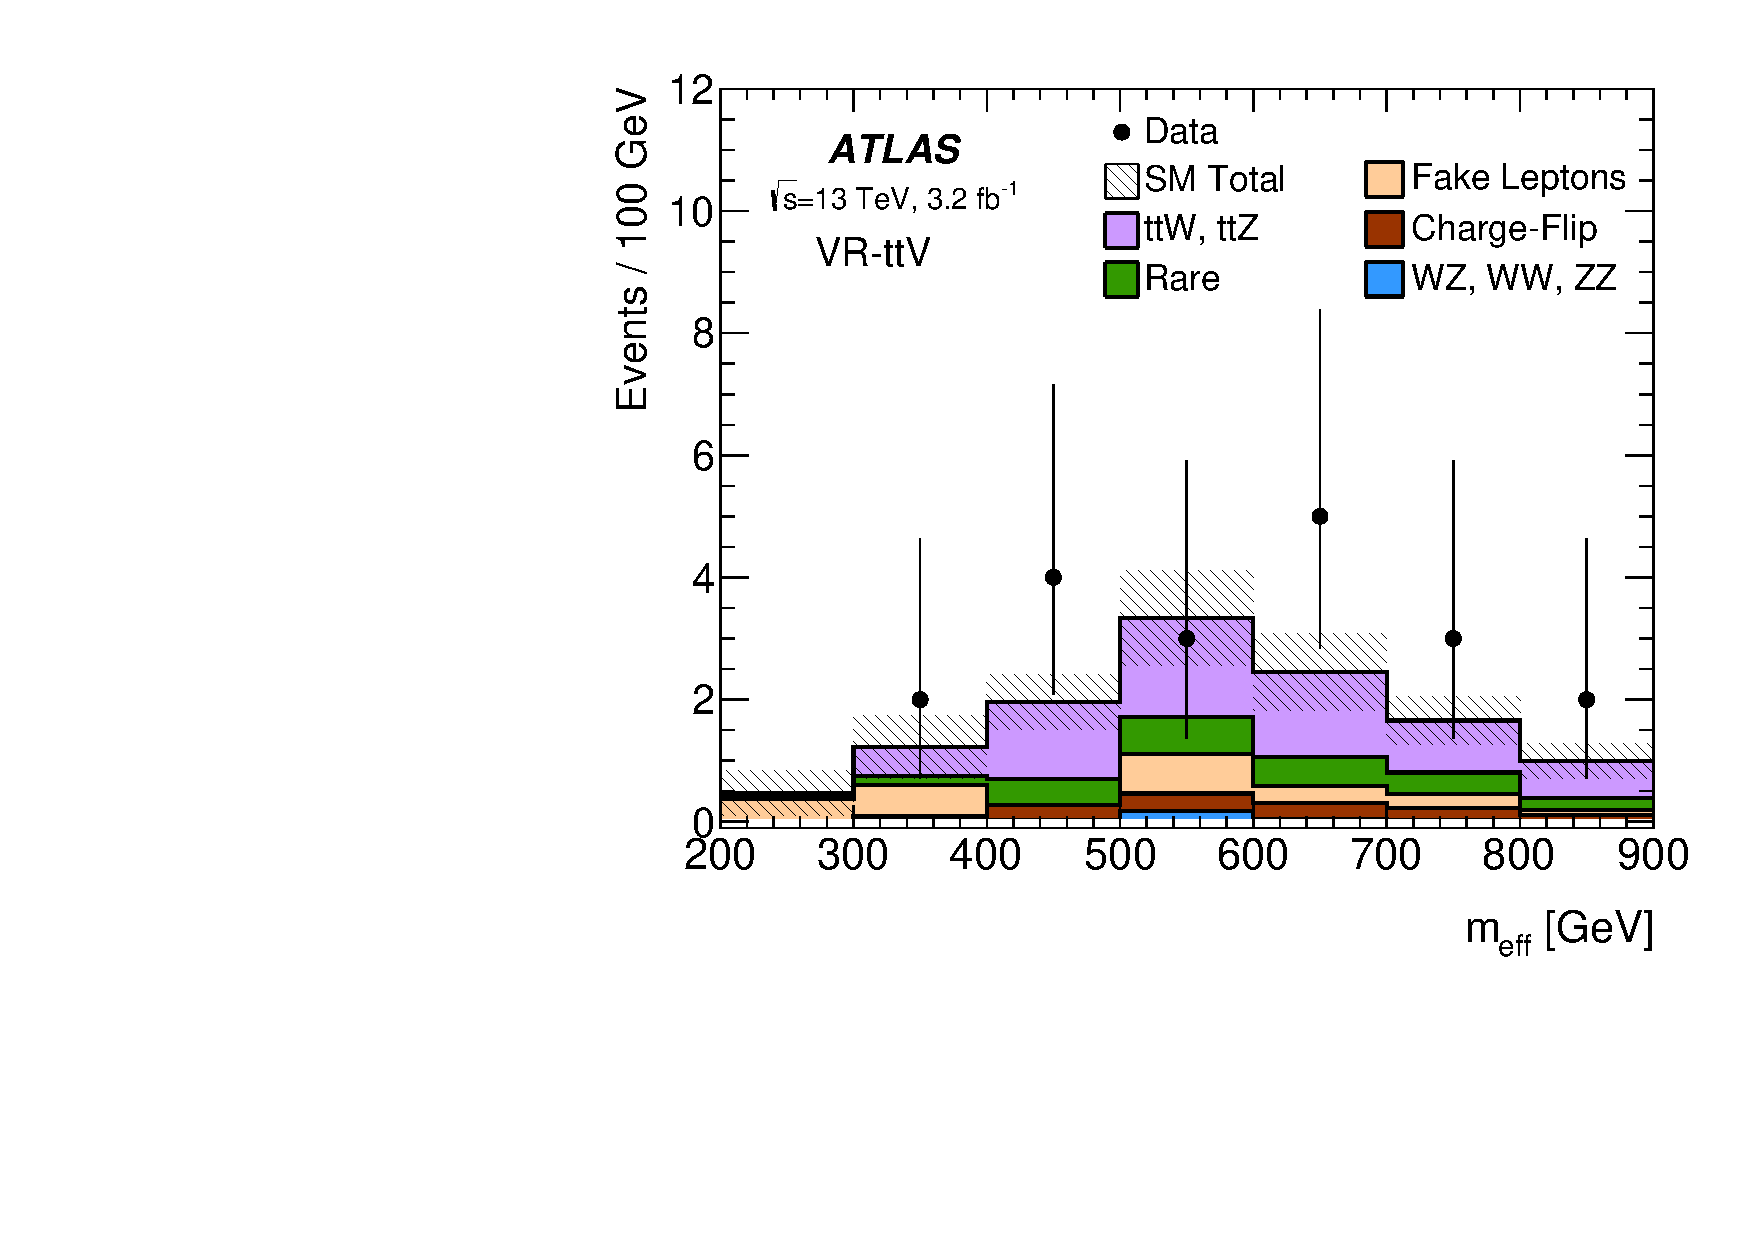
\includegraphics[width=\textwidth]{FIGURES/CONF_ttV2bInclVR.pdf}
\caption{}\label{fig:VRe}\end{subfigure}
\begin{subfigure}[t]{0.46\textwidth}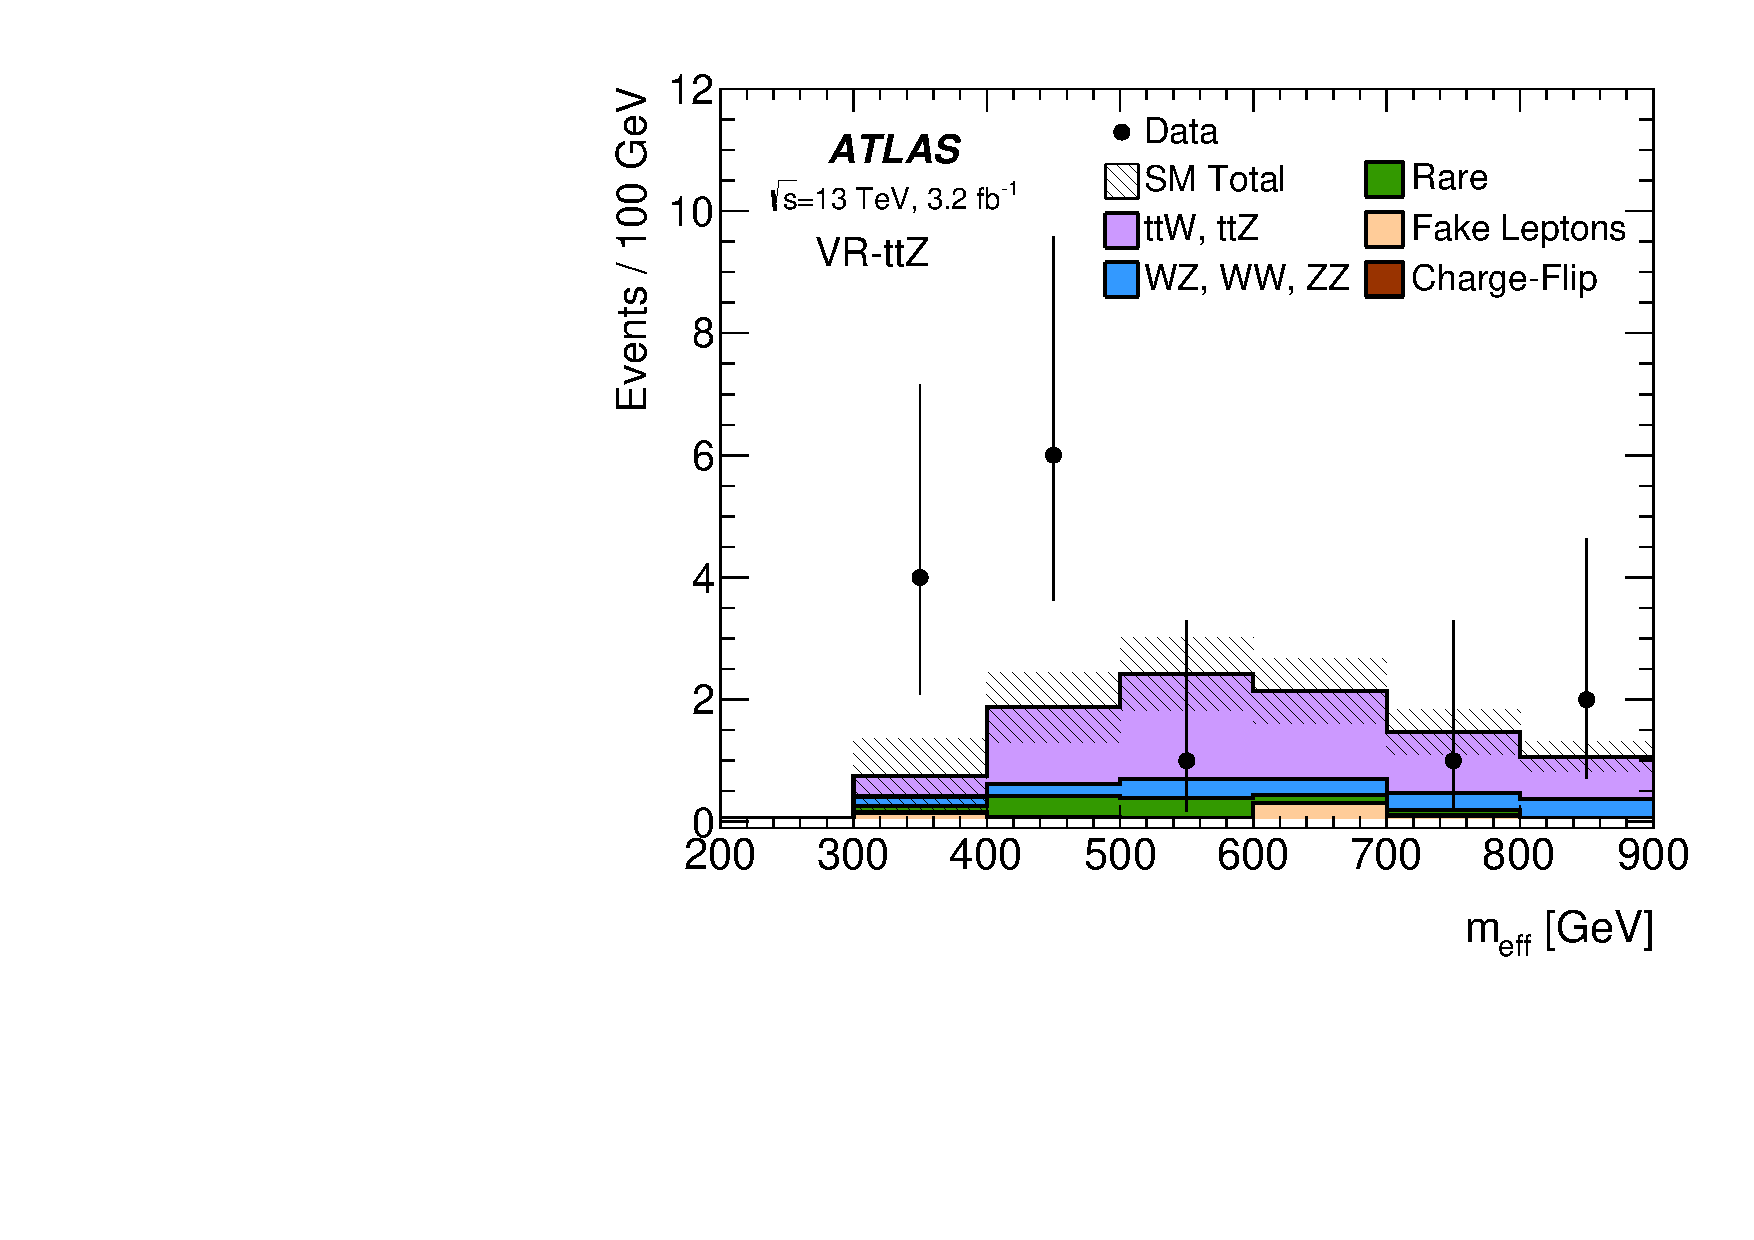
\includegraphics[width=\textwidth]{FIGURES/CONF_ttZ1bInclVR.pdf}
\caption{}\label{fig:VRf}\end{subfigure}
\caption{Distributions of kinematic variables after a SS/3L selection 
including (a), (b) $\met>\SI{60}{GeV}$ and $N_\text{jet}^{25}\ge 2$, 
(c) a $b$-jet veto and $80<m_{\ell\ell}<\SI{100}{GeV}$, 
and (d), (e), (f) distributions in the validation regions. 
The statistical uncertainties in the background prediction are included in the uncertainty band, 
as well as the theory uncertainties for the backgrounds with prompt SS/3L, 
and the full systematic uncertainties for data-driven backgrounds. 
The last bin includes overflows. 
The ``Fake leptons'' category corresponds to FNP leptons (see text), 
and the ``Rare'' category contains the contributions from associated production of $\ttbar$ with $h/WW/t/\ttbar$, 
as well as $tZ$, $Wh$, $Zh$, and triboson production. 
The lower part of the figures (a)--(d) shows the ratio of data to the background prediction.}
\label{fig:Validation_plots} 
\end{figure} 
